% TikZ redraw for exercise 2-27
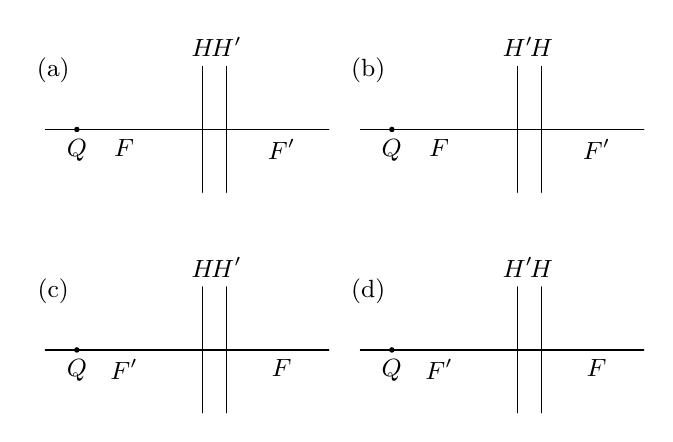
\begin{tikzpicture}[font=\small,line cap=round,line join=round]
\foreach\x/\y/\name/\swap/\reverse in {0/0/a/0/0,4/0/b/0/1,0/-2.8/c/1/0,4/-2.8/d/1/1}{\begin{scope}[shift={(\x,\y)}]\draw(-2,0)--(1.6,0);\ifnum\reverse=0\def\h{0}\def\hh{.3}\else\def\h{.3}\def\hh{0}\fi\draw(\h,-.8)--(\h,.8)node[above]{$H$};\draw(\hh,-.8)--(\hh,.8)node[above]{$H'$};\node at(-1.9,.75){(\name)};\node[below]at(-1.6,0){$Q$};\fill(-1.6,0)circle(1pt);\ifnum\swap=0\node[below]at(-1,0){$F$};\node[below]at(1,0){$F'$};\else\node[below]at(-1,0){$F'$};\node[below]at(1,0){$F$};\fi\end{scope}}
\end{tikzpicture}
